%!TEX root =../mapp-challenge-18-game-book.tex
% ^ leave for LaTeXTools build functionality

\phChapterWorksheet{When Push Comes to Shove}{Main Puzzle 2}

\newcommand{\mappBoxRow}[2]{
  \fill[color=lightgray] #1 rectangle #2;
  \draw[step=1]          #1 grid #2;
}

% http://oeis.org/A000041 number of partitions
% http://oeis.org/A000009 number of odd/distinct partitions

While training your \mappMobimon{} on Road \(\sqrt{9^2+12^2}\), you are
approached
by \textbf{Dockworker Dave}, who challenges you to a \mappMobidot{} battle!
Of course you accept... turning him down would be \textbf{rude},
don't you think?

It's a close match, but you win! As Dave gives you your victory money, he
tells you about a group of \textbf{Tattarat} \mappMobimon{} that infest the
warehouse he works in. These obnoxious critters like to
\textbf{rearrange the boxes} in his warehouse, so Dave cuts you a deal.
He'll let you catch a Tattarat for your team, but only if you help
him reorganize his boxes.

The boxes in the warehouse must be \textbf{stacked} so that
each row of boxes is always pressed up against the \textbf{left wall} of the
warehouse, and each row of boxes must have the \textbf{same or less boxes} than
every lower row.

Other than that, it's up to you. For example, there are \textbf{seven}
different ways to stack \textbf{five} boxes.

\begin{center}
  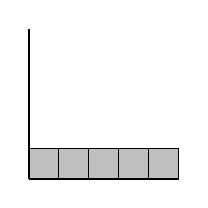
\begin{tikzpicture}[x=0.15in,y=0.15in]
    \mappBoxRow{(0,0)}{(5,1)}

    \draw[thick] (0,0) -- (0, 5);
    \draw[thick] (0,0) -- (5, 0);
  \end{tikzpicture}
  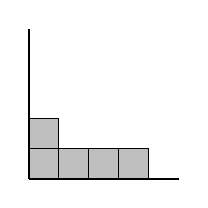
\begin{tikzpicture}[x=0.15in,y=0.15in]
    \mappBoxRow{(0,0)}{(4,1)}
    \mappBoxRow{(0,1)}{(1,2)}

    \draw[thick] (0,0) -- (0, 5);
    \draw[thick] (0,0) -- (5, 0);
  \end{tikzpicture}
  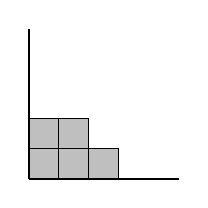
\begin{tikzpicture}[x=0.15in,y=0.15in]
    \mappBoxRow{(0,0)}{(3,1)}
    \mappBoxRow{(0,1)}{(2,2)}

    \draw[thick] (0,0) -- (0, 5);
    \draw[thick] (0,0) -- (5, 0);
  \end{tikzpicture}
  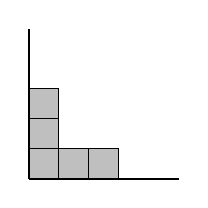
\begin{tikzpicture}[x=0.15in,y=0.15in]
    \mappBoxRow{(0,0)}{(3,1)}
    \mappBoxRow{(0,1)}{(1,2)}
    \mappBoxRow{(0,2)}{(1,3)}

    \draw[thick] (0,0) -- (0, 5);
    \draw[thick] (0,0) -- (5, 0);
  \end{tikzpicture}
  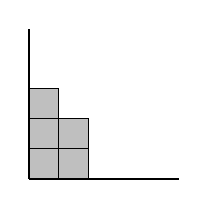
\begin{tikzpicture}[x=0.15in,y=0.15in]
    \mappBoxRow{(0,0)}{(2,1)}
    \mappBoxRow{(0,1)}{(2,2)}
    \mappBoxRow{(0,2)}{(1,3)}

    \draw[thick] (0,0) -- (0, 5);
    \draw[thick] (0,0) -- (5, 0);
  \end{tikzpicture}
  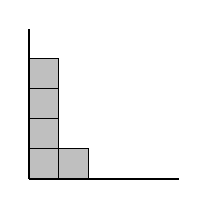
\begin{tikzpicture}[x=0.15in,y=0.15in]
    \mappBoxRow{(0,0)}{(2,1)}
    \mappBoxRow{(0,1)}{(1,2)}
    \mappBoxRow{(0,2)}{(1,3)}
    \mappBoxRow{(0,3)}{(1,4)}

    \draw[thick] (0,0) -- (0, 5);
    \draw[thick] (0,0) -- (5, 0);
  \end{tikzpicture}
  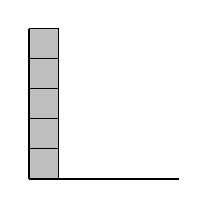
\begin{tikzpicture}[x=0.15in,y=0.15in]
    \mappBoxRow{(0,0)}{(1,1)}
    \mappBoxRow{(0,1)}{(1,2)}
    \mappBoxRow{(0,2)}{(1,3)}
    \mappBoxRow{(0,3)}{(1,4)}
    \mappBoxRow{(0,4)}{(1,5)}

    \draw[thick] (0,0) -- (0, 5);
    \draw[thick] (0,0) -- (5, 0);
  \end{tikzpicture}
\end{center}

The dockworker notices your good work.
``Hey, didya say you were aiming to become one of them \mappMobimon{}
Champions? Maybe you're smart enough to solve this \textbf{puzzle} for me
then.'' It seems that if you can count the following different combinations
of stacked boxes, you'll be able to reveal a \textbf{hidden message} by
converting the numbers to appropriate letters (A=1, B=2, and so on).

\begin{multicols}{2}
  \begin{itemize}
    \item %M=13
      The number of ways you can stack either \(2\) or \(6\) boxes.
    \item %O=15
      The number of ways you can stack \(12\) boxes, if every row must
      contain an odd number.
    \item %U=21
      The number of ways you can stack \(8\) boxes, if every row must contain
      less than eight.
    \item %S=19
      The number of ways you can stack up to \(5\) boxes. (An empty room
      counts as one way...)
    \item %E=5
      The number of ways you can stack \(4\) boxes.
  \end{itemize}
\columnbreak
  \begin{itemize}
    \item %T=20
      The number of ways you can stack \(8\) boxes, if every row must contain
      less than seven.
    \item %R=18
      The number of ways you can stack \(13\) boxes, if every row must have
      less boxes than the row below it.
    \item %A=1
      The number of ways you can stack \(42\) boxes, if you can only use one
      row.
    \item %P=16
      The number of ways you can stack \(1\) or \(12\) boxes, if every row must
      have a unique number of boxes.
  \end{itemize}
\end{multicols}


%%SOLUTION%%%
% MOUSETRAP %
%%%%%%%%%%%%%


% Old unused text:

% For example, this configuration looks solid.
% \begin{center}
%   \begin{tikzpicture}
%     \fill[color=lightgray] (0,0) rectangle (4,1);
%     \draw             (0,0) grid (4,1);
%     \fill[color=lightgray] (0,1) rectangle (3,2);
%     \draw             (0,1) grid (3,2);
%     \fill[color=lightgray] (0,2) rectangle (1,3);
%     \draw             (0,2) grid (1,3);
%
%     \draw[thick] (0,0) -- (0, 4);
%     \draw[thick] (0,0) -- (5, 0);
%   \end{tikzpicture}
% \end{center}
%
% But this one isn't so great.
% Not only are the boxes not all pushed to the left, but how are some of them
% floating in the air like that anyway? That's just not right.
%
% \begin{center}
%   \begin{tikzpicture}
%     \fill[color=lightgray] (0,0) rectangle (2,1);
%     \draw             (0,0) grid (2,1);
%     \fill[color=lightgray] (1,1) rectangle (4,2);
%     \draw             (1,1) grid (4,2);
%     \fill[color=lightgray] (2,2) rectangle (3,3);
%     \draw             (2,2) grid (3,3);
%
%     \draw[thick] (0,0) -- (0,4);
%     \draw[thick] (0,0) -- (5,0);
%   \end{tikzpicture}
% \end{center}
%




%%% Local Variables:
%%% mode: latex
%%% TeX-master: "../mapp-challenge-18-game-book"
%%% End:
